\documentclass[11pt]{beamer}
\usetheme{metropolis}           % Use metropolis theme

\usepackage{sansmathaccent}
\pdfmapfile{+sansmathaccent.map}

% Libraries for the tree
\usepackage{pgf}
\usepackage{tikz}
\usetikzlibrary{arrows,automata}
\usepackage[latin1]{inputenc}

\usepackage{mathtools}
\usepackage{graphicx}
\usepackage{subcaption}
\usepackage{amsmath}

% Create argmax
\DeclareMathOperator*{\argmax}{argmax}

% \graphicspath{ {/home/chrishittner/Desktop/} }

\title{A Brief Glimpse at Machine Learning}
\subtitle{With Demos and Explanations}
\author{Christopher Hittner}
\date{11 October 2017}
%\institute{Centre for Modern Beamer Themes}
\begin{document}
\maketitle

\section{What is Machine Learning?}

\begin{frame}{Machine Learning}
\begin{itemize}
    \item Teaching computers to learn without explicit training.
    \item Making predictions about data.
    \begin{itemize}
        \item ex: Predicting movie ratings.
    \end{itemize}
    \item Learning to perform tasks.
    \begin{itemize}
        \item ex: Game playing AI for games such as Chess, Go, etc.
    \end{itemize}
\end{itemize}
\end{frame}

\begin{frame}{Notable AI/ML Applications}
\begin{itemize}
    \item Game Playing AI
    \begin{itemize}
        \item Deep Blue (1997)
        \item AlphaGo (2016)
    \end{itemize}
    \item Natural Language Processing
    \begin{itemize}
        \item Cleverbot (1997)
        \item Eliza (1966)
    \end{itemize}
    \item Back-end
    \begin{itemize}
        \item Google: RankBrain
        \item Facebook: Facial Recognition
    \end{itemize}
\end{itemize}
\end{frame}


\begin{frame}{Learning Problems}
\begin{itemize}
    \item Classification
    \begin{itemize}
        \item Learning to categorize data.
    \end{itemize}

    \item Regression
    \begin{itemize}
        \item Learning to represent continuous functions.
        \item Representing more precise probability functions.
    \end{itemize}

    \item Clustering
    \begin{itemize}
        \item Categorizing data where the categories are unknown.
    \end{itemize}
\end{itemize}
\end{frame}

\begin{frame}{Types of Learning}
\begin{itemize}
    \item Supervised Learning
    \begin{itemize}
        \item Given example inputs and outputs, learn to predict/approximate the data.
    \end{itemize}
    \item Unsupervised Learning
    \begin{itemize}
        \item Given only input data, learn to classify it.
    \end{itemize}
    \item Reinforcement Learning
    \begin{itemize}
        \item Learner receives stimulus while interacting with environment.
    \end{itemize}
\end{itemize}
\end{frame}

\section{Types of Machine Learning}

\begin{frame}{Classification}
% Demo is in ./classification/class.py
\begin{itemize}
    \item Given a set of items with known categories, classify new items.
    \begin{itemize}
        \item With a given set of item-category pairs, learn a function to match these pairs.
        \item Using classifier, categorize new items into categories.
    \end{itemize}
    \begin{alertenv}
        \item Naive Bayes
    \end{alertenv}
    \begin{itemize}
        \item Statistical classification method based on Bayes' Theorem
        \item For n features $F = \{F_1, F_2, \ldots, F_n\}$, we seek k such that \\
                \[\argmax_k P(C_k | F) = P(C_k) \prod_{i=0}^{n} P(F_i | C_k)\]
        \item If $C$ is a continuous set, then P can be replaced with density function p.
    \end{itemize}
\end{itemize}
\end{frame}

\begin{frame}{Regression}
% Demo is in ./regression/reg.py
\begin{itemize}
    \item Given a dataset, we seek a function to fit the data points.
    \begin{itemize}
        \item Adjust function such that it more accurately represents the data.
    \end{itemize}
    \begin{alertenv}
        \item Linear Regression
    \end{alertenv}
    \begin{itemize}
        \item Given a system of linear equations, determine a best fit via a system of equations.
        \item To approximate $X \vec{c} = \vec{y}$, we compute $\vec{c}$ that solves $X^T X \vec{c} = X^T \vec{y}$
    \end{itemize}
    \begin{alertenv}
        \item Logistic Regression
    \end{alertenv}
    \begin{itemize}
        \item Categorical regression model used to predict probability.
        \item We seek to learn parameter $\vec{\theta}$ such that \[P(x) = \frac{1}{1 + e^{-\vec{\theta}^T \vec{x}}}\]
    \end{itemize}
\end{itemize}
\end{frame}

\begin{frame}{Clustering}
% Demo is in video_cluster
\begin{itemize}
    \item Given a set of data, group it into categories.
    \begin{itemize}
        \item We seek to determine which items are alike.
    \end{itemize}
    \begin{alertenv}
        \item K-Means Clustering
    \end{alertenv}
    \begin{itemize}
        \item Centroid clustering algorithm.
        \item Cluster data into k categories.
        \item Points belong to category with closest mean.
    \end{itemize}
    \begin{alertenv}
        \item DBSCAN
    \end{alertenv}
    \begin{itemize}
        \item Density-Based Spatial Clustering of Applications with Noise
        \item Groups points that are close to one another.
        \item Can classify non-linearly separable clusters.
    \end{itemize}
\end{itemize}
\end{frame}

\section{Deep Learning/Neural Networks}

\begin{frame}{Deep Learning}
\begin{itemize}
    \item Form of learning meant to learn features.
    \begin{itemize}
        \item Generally associated with neural networks.
        \item Use of gradient descent to train computation layers.
    \end{itemize}
    \item Neural Network: Computational model consisting of layers of neurons.
    \begin{itemize}
        \item Feedforward NN
        \begin{itemize} \item Output computed sequentially. \end{itemize}
        \item Convolutional NN
        \begin{itemize} \item Computing layers from sections of image. \end{itemize}
        \item Recurrent NN
        \begin{itemize} \item Layer outputs computed recursively. \end{itemize}
    \end{itemize}
\end{itemize}
\end{frame}

\begin{frame}{Neural Networks: Learning Algorithms}
\begin{itemize}
    \begin{alertenv}
        \item Backpropagation
    \end{alertenv}

    \begin{itemize}
        \item Using gradient descent across layers to minimize a loss function.
    \end{itemize}

    \item Hebbian Learning
    \begin{itemize}
        \item Increase activation due to given inputs to associate data with stimuli.
    \end{itemize}

    \item Kohonen Self-Organizing Map
    \begin{itemize}
        \item Network type used for mapping from high dimensional data to lower dimension.
    \end{itemize}

\end{itemize}
\end{frame}

\section{Decision Trees}

\begin{frame}{Decision Trees}
\begin{itemize}
    \item Given a system with rules, we seek to optimize a score.
    \begin{itemize}
        \item We want to optimize in long term, not only in short term.
        \item Furthermore, we recognize that oppsition can exist.
        \item With information on the system, we can create trees of all possible evaluations.
    \end{itemize}
\end{itemize}

\begin{center}
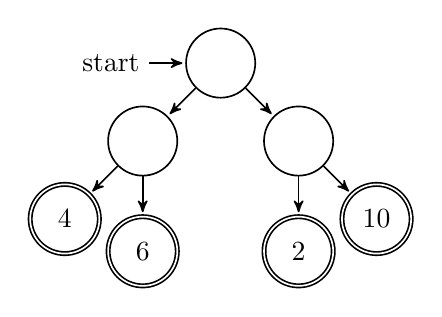
\begin{tikzpicture}[->,>=stealth',shorten >=1pt,auto,node distance=1.4cm,
                    semithick]

\node[initial,state] (A) [] {};
\node[state] (B) [below left of=A]  {};
\node[state] (C) [below right of=A] {};
\node[state,accepting] (D) [below left of=B]  {4};
\node[state,accepting] (E) [below of=B] {6};
\node[state,accepting] (F) [below of=C]  {2};
\node[state,accepting] (G) [below right of=C] {10};

\path
    (A) edge [] node {} (B)
        edge [] node {} (C)
    (B) edge [] node {} (D)
        edge [] node {} (E)
    (C) edge [] node {} (F)
        edge [] node {} (G)
;
\end{tikzpicture}

Game: Take turns choosing an edge to traverse. One player maximizes, the other minimizes.
\end{center}

\end{frame}

\begin{frame}{Decision Trees}
% Demo is in ./mcarlo/play.py
\begin{itemize}
    \item Minimax Trees
    \begin{itemize}
        \item Traverse a tree and find the best possible path.
        \item Generally bounded due to large search space.
        \item Can be pruned to ignore solutions (Alpha-Beta Pruning)
    \end{itemize}
    \begin{alertenv}
        \item Monte Carlo Trees
    \end{alertenv}
    \begin{itemize}
        \item Random search of decision tree to estimate best path.
        \item Can prioritize unexplored and favorable solutions during search.
        \item Allows deeper search than minimax due to random search.
    \end{itemize}
\end{itemize}
\end{frame}

\section{Natural Language Processing}

\begin{frame}{Natural Language Processing}
\begin{itemize}
    \item Given some spoken or written information, we seek to deduce new information from it.
    \begin{itemize}
        \item Detecting meaning in a segment of text.
        \item Determining relevance of information.
        \item Converting between speech and text.
    \end{itemize}
    \begin{alertenv}
    \item Word2Vec
    \end{alertenv}
    \begin{itemize}
        \item Algorithm for computing similarity between words.
        \item Given a set of sentences, determine representative vectors such that similarity is equal to dot product.
    \end{itemize}
    \begin{alertenv}
    \item Lesk Algorithm
    \end{alertenv}
    \begin{itemize}
        \item Predicts approximate definition of word in context.
        \item Chooses word definition with most overlap with sentence
    \end{itemize}
\end{itemize}
\end{frame}

\section{Genetic Algorithms}

\begin{frame}{Genetic Algorithms}
\begin{itemize}
    \item We seek to determine optimal parameters in a given scenario.
    \begin{itemize}
        \item Gradient unavailable; `fitness' function $F(\vec{\theta})$ has non-trivial gradient.
    \end{itemize}
    \item Solution: Artificial Selection
    \begin{itemize}
        \item Evaluate samples and select best ones.
        \item Use genetic operators to improve genes (mutation, crossover, selection)
        \item Breed an optimal `gene'.
    \end{itemize}
\end{itemize}
\end{frame}

\begin{frame}{Further Reading}
\begin{itemize}
    \item \textit{On the Computational Power of Neural Nets} (1995)
    \item \textit{Neural Network Design} (1996)
    \item \textit{ImageNet Classification with Deep Convolutional Neural Networks} (2012)
    \item \textit{Generative Adversarial Networks} (2014)
    \item \textit{Mastering the game of Go with deep neural networks and tree search} (2016)
\end{itemize}
\end{frame}

\end{document}
